\documentclass[11pt,en]{elegantpaper}
\usepackage{graphicx}
\usepackage{float}
\usepackage{neuralnetwork}
\title{The Classification and Prediction of Diabetes Dataset}
\author{Wangzhihui Mei 2019124044 \\ Hongyi Huang 201912xxxx \\ Zijia He 201912xxxx \\ Chang Xu 201912xxxx}
\institute{CCNU-UOW JI}

\begin{document}

\maketitle



\section{Introduction}
This dataset is originally from the National Institute of Diabetes and Digestive and Kidney Diseases. The objective of the dataset is to diagnostically predict whether or not a patient has diabetes, based on certain diagnostic measurements included in the dataset. Several constraints were placed on the selection of these instances from a larger database. In particular, all patients here are females at least 21 years old of Pima Indian heritage.

There are 8 features:\\
\begin{itemize}
    \item Number of times pregnant
    \item Plasma glucose concentration a 2 hours in an oral glucose tolerance test
    \item Diastolic blood pressure (mm Hg)
    \item 2-Hour serum insulin (mu U/ml)
    \item Triceps skin fold thickness (mm)
    \item Body mass index (weight in kg/$(height in m)^2$)
    \item Diabetes pedigree function
    \item Age (years)
\end{itemize}

And 1 label (response variable). These data are collected from actual patients and represent a task, 
usually performed by a human doctor, with the purpose of identifying the patients most likely to have
diabetes in order to propose preventive measures. \\
Next, we conducted some comparative studies on these data, we can get a table:\\
\begin{figure}[H]
    \centering
    
\includegraphics[scale=0.6]{figure/1.PNG}  
\end{figure}

\begin{figure}[H]
    \centering
    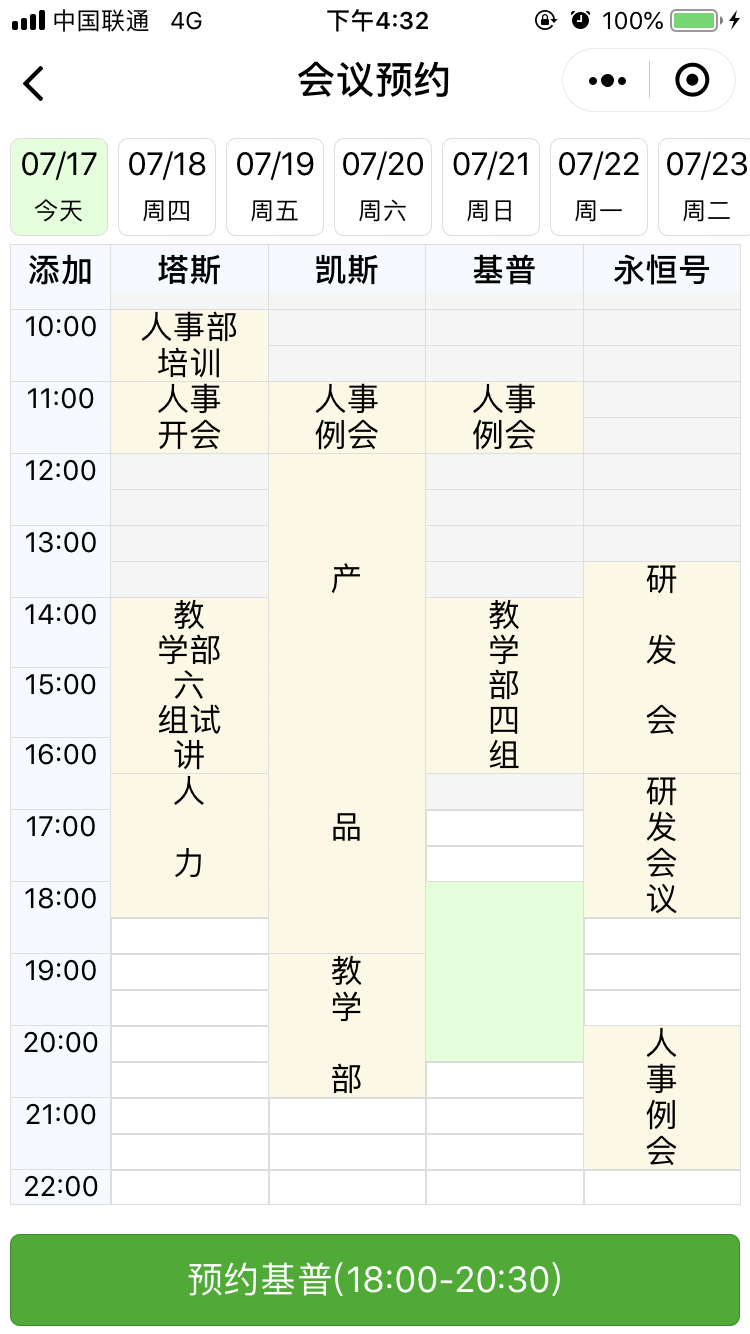
\includegraphics[scale=0.6]{figure/2.PNG}  
\end{figure}



\section{Data preparation}
There are 8 features (explanatory variables) and 1 label (response variable). These data are collected from actual patients and represent a task, usually performed by a human doctor, with the purpose of identifying the patients most likely to have diabetes in order to propose preventive measures.Some data values are 0, which is impossible, because these physical quantities cannot be 0 (for living people). Therefore, this has told us that we need to estimate these five columns. The scope of other variables seems to be reasonable.Next, we can calculate the relevant values to see the relationship between the characteristics and the results. Of course, correlation does not mean causality, but because we are building a linear model, correlation features may be useful for learning the mapping between patient information and whether they have diabetes.In problems with a large number of features, we can use relevant thresholds to delete variables. In this case, we may want to keep all variables and let the model decide which ones are related.In this brief exploratory data analysis, we learned about the two main aspects of data sets that can be used for modeling. First, we need to enter missing values in several columns, because these values are physically impossible. We can use the median method as a simple and effective way to fill the value of 0. We also learned that there is a correlation between features and responses, although the correlation is not strong. In addition, all features are at least slightly positively correlated with the result (whether or not the patient has diabetes).Next, in order to facilitate testing and training, we randomly select 75\% of the data set for training and 25\% of the data set for testing.

% \begin{figure}[H]
% \centering
% 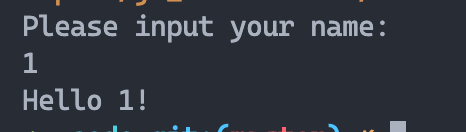
\includegraphics[width=0.8\textwidth]{figure/1-2.png}
% \caption{Correlation}
% \end{figure}

% \begin{figure}[H]
% \centering
% 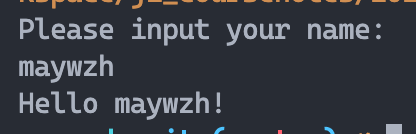
\includegraphics[width=6in]{figure/1-1.png}
% \caption{Data filled with missing values}
% \end{figure}

\subsection{whether the pregnancy column is continuous or categorical variable}
We need to answer whether the Pregnancy is something is being measured or counted. Since, pregnancy is neither Counted or Measured, we should not be considering the Pregnancy column as Numerical and we should consider the same as Categorical.

Additional Input - Categorical can be further divided into 'Nominal' or 'Ordinal'.
\begin{itemize}
    \item Nominal - There is no order in the values
    \item Ordinal - There is Order in the values ( like Good , Bad , Poor )
\end{itemize}

\subsection{Handleing with missing data}
Firstly we cannot simply ignore missing values in a dataset. We must handle them in some way for the very practical reason that most algorithms do not accept missing values.

"Common sense" is not sensible here.From my experience the 2 most commonly recommended ways of dealing with missing data actually are not accurate.
\begin{itemize}
    \item Dropping observations that have missing values
    \item Imputing the missing values based on other observations
\end{itemize}

Dropping missing values is sub-optimal because when we drop observations, we drop information.

The fact that the value was missing may be informative in itself.We need to understand business deeper to uncover why this information is missing in real world problems.In real time problems we need to make predictions even if some of the features are missing !!!.

Imputing missing values is sub-optimal because the value was originally missing but you filled it in, which always leads to a loss in information, no matter how sophisticated our imputation method is.

"Missingness" is almost always informative in itself, and we should tell our algorithm if a value was missing.Even if we build a model to impute our values, we are not adding any real information. You’re just reinforcing the patterns already provided by other features.

\subsubsection{Strategies}

We should never insert mean, mode, median, max, min or anything else for missing values. That is, avoid deterministic imputation even though it is widely used and available in most software packages. It underestimates and distorts the statistical regularities (e.g., underestimates variance is one example) present in the data sample.

If the data records are MCAR Then you can delete records with missing data.

If the data records are MCAR, then sometimes you can stochastically impute the missing values rather than deterministically impute them. So this means that if you specify the marginal probability distribution of a missing value as Gaussian with some known mean and some known variance then you can sample from that distribution to impute values into the data set. We need to be careful and do some additional research and analysis on data ,understand the business completely and take a judicious decision.

If the data is MAR then an algorithm such as Expectation Maximization can be used to handle the missing observations.

If the data is MNAR we can include binary indicators in the data record which explicitly identify when a variable is not observable. The challenge with this approach is that a highly nonlinear model needs to be designed to properly integrate this information in an appropriate manner. This might work in a machine learning algorithm where the binary indicators "disconnect" the influence of predictors which are not observable. Consequently, the MNAR theory (i.e., the theory of the joint distribution of the complete data record and missing data pattern) is instantiated in the learning machine's probabilistic model of its statistical environment.

\subsubsection{Missing numeric data}
For missing numeric data, we should flag and fill the values.

Flag the observation with an indicator variable of missingness.
Secondly fill the original missing value with 0 just to meet the technical requirement of no missing values.
By using this technique of flagging and filling, we are essentially allowing the algorithm to estimate the optimal constant for missingness, instead of just filling it in with the mean.

\subsubsection{Missing categorical data}
The best way to handle missing data for categorical features is to simply label them as ’Missing’!

We are essentially adding a new class for the feature.
This tells the algorithm that the value was missing.
This also gets around the technical requirement for no missing values.

\subsection{Dataset Analysis}

\subsubsection{Type of data}
\begin{figure}[H]
    \centering
    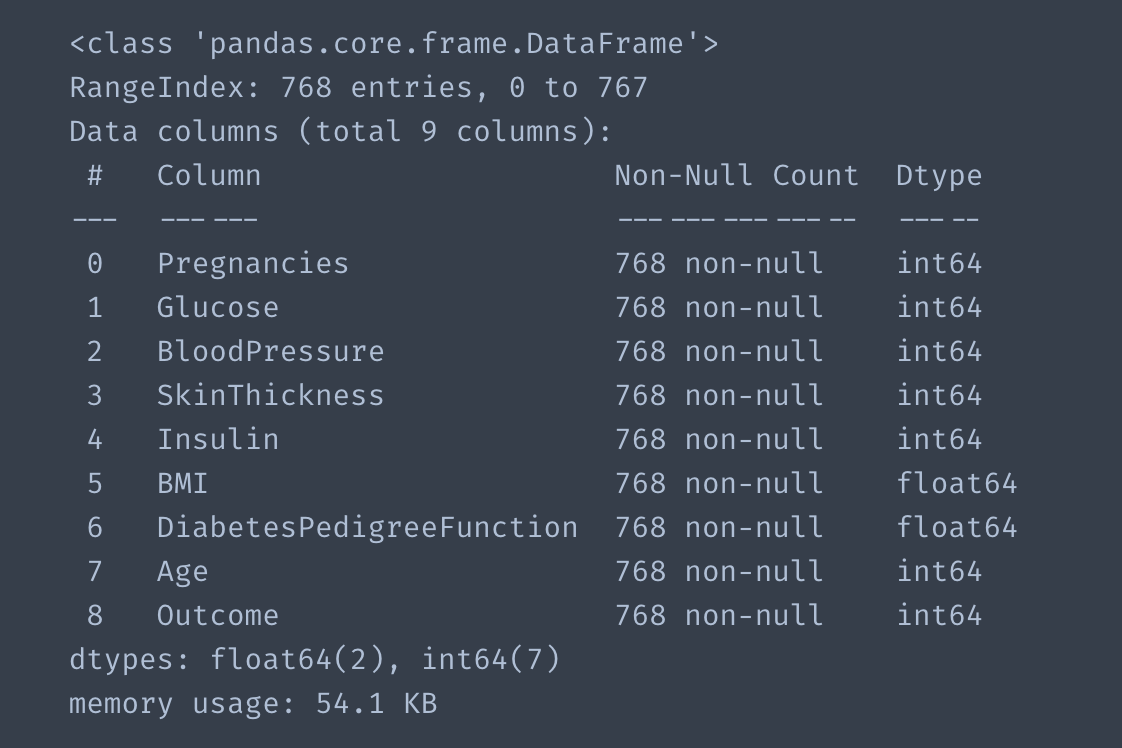
\includegraphics[width=0.7\textwidth]{figure/f0.png}
    \caption{Type of data}
\end{figure}

\subsubsection{The Ratio of Positive and Negative}
\begin{figure}[H]
    \centering
    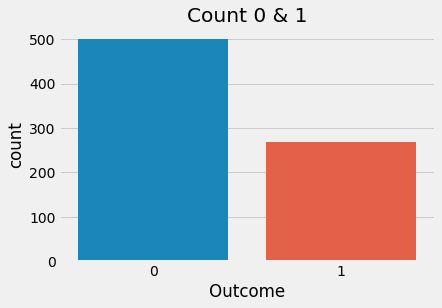
\includegraphics[width=0.8\textwidth]{figure/f1.png}
    \caption{Correlation}
\end{figure}
\subsubsection{The Relevance of Features}
\begin{figure}[H]
    \centering
    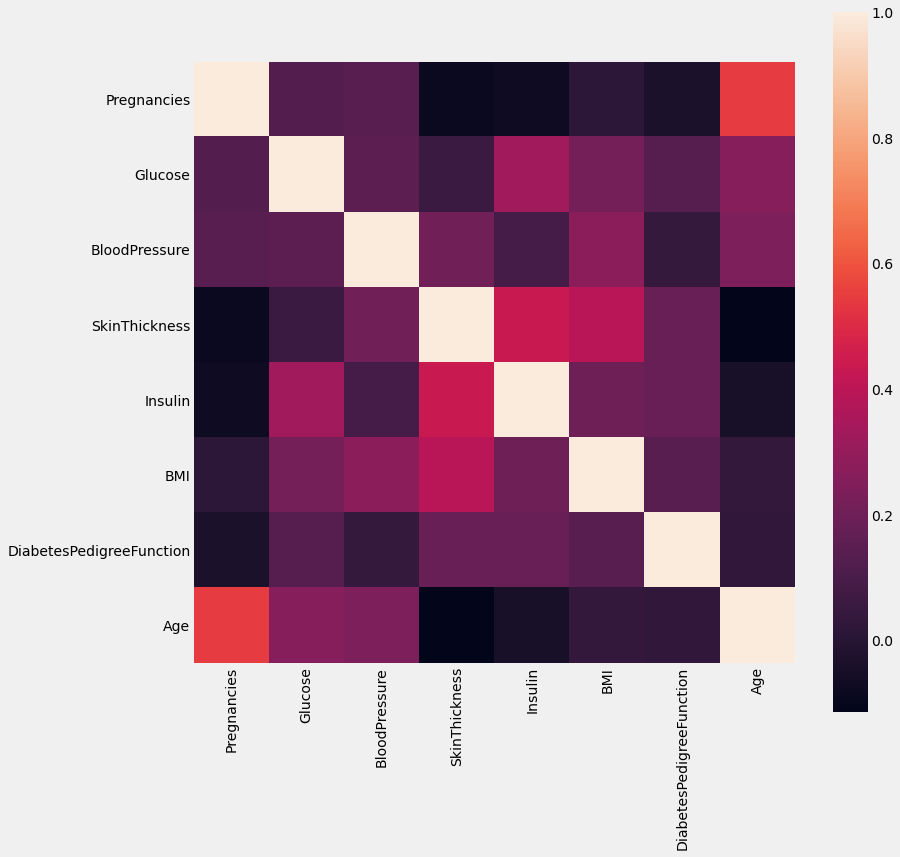
\includegraphics[width=0.8\textwidth]{figure/relevance-data}
    \caption{Correlation}
\end{figure}
\subsubsection{Analysis of Diabetic Cases}
\begin{figure}[H]
    \centering
    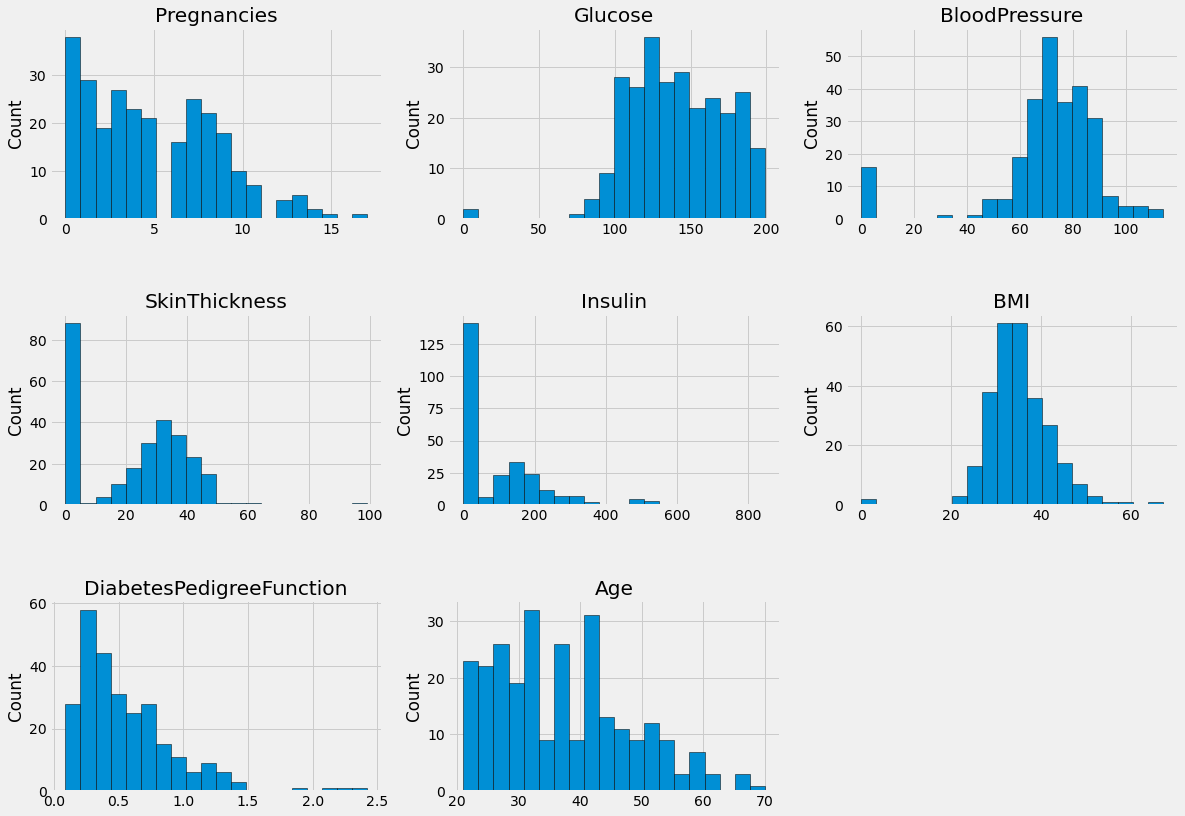
\includegraphics[width=0.8\textwidth]{figure/f2.png}
    \caption{Analysis of Diabetic Cases}
\end{figure}

\subsubsection{Analysis of Non-Diabetic Cases}
\begin{figure}[H]
    \centering
    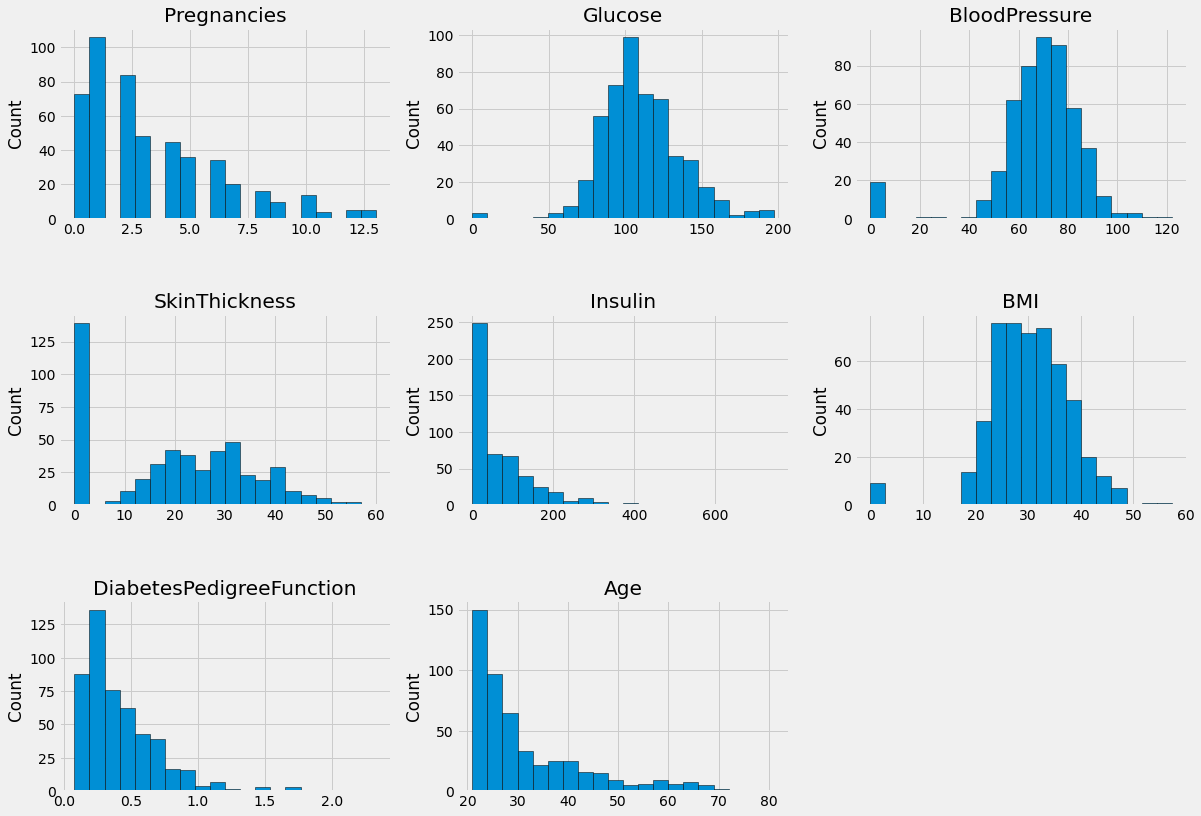
\includegraphics[width=0.8\textwidth]{figure/f3.png}
    \caption{Analysis of Diabetic Cases}
\end{figure}

\subsubsection{Effects of Pregnancies and Glucose on diabetes}
\begin{figure}[H]
    \centering
    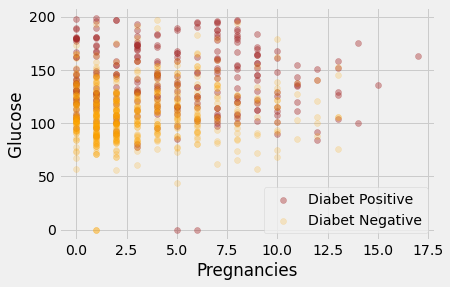
\includegraphics[width=0.8\textwidth]{figure/f4.png}
    \caption{Effects of Pregnancies and Glucose on diabetes}
\end{figure}

\subsubsection{Effect of Pregnancies and Age on diabetes}
\begin{figure}[H]
    \centering
    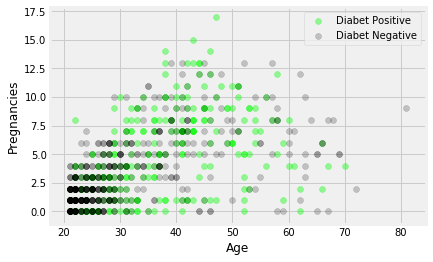
\includegraphics[width=0.8\textwidth]{figure/f5.png}
    \caption{Effect of Pregnancies and Age on diabetes}
\end{figure}

\subsubsection{Effects of Insulin and Glucose on diabetes}
\begin{figure}[H]
    \centering
    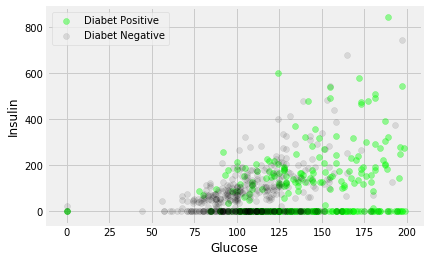
\includegraphics[width=0.8\textwidth]{figure/f6.png}
    \caption{Effects of Insulin and Glucose on diabetes}
\end{figure}



\section{Classifiers}
An important purpose of model verification is to select the most suitable model. For supervised learning, we hope that the model has a strong generalization ability for unknown data, so a model verification process is needed to reflect the different models for the unknown. The performance of the data.

First, we use training accuracy (using all data for training and testing) to measure the performance of the model. This method will cause the model to overfit; to solve this problem, we divide all the data into training and test sets. , We use the training set for model training, and the obtained model is then used to test the model to measure the predictive performance of the model. This measure is called test accuracy, which can effectively avoid overfitting.

One disadvantage of test accuracy is that its sample accuracy is a high variance estimate, so the sample accuracy will depend on different test sets and its performance will vary.

We use K-fold Cross Validation to train classifiers.
\begin{figure}[H]
    \centering
    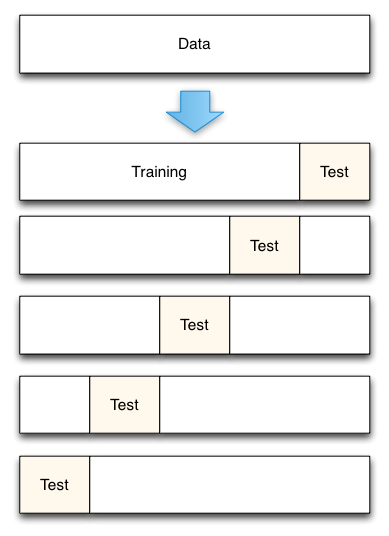
\includegraphics[width=0.5\textwidth]{figure/cross_validation_diagram.png}
    \caption{K-fold Cross Validation}
\end{figure}

\subsection{Logistic Regression Classification}
\subsubsection{Description}
As the name suggests, it is actually a variant of the regression class method. The core of the regression method is to find the most suitable parameters for the function, so that the value of the function is closest to the value of the sample. For example, linear regression (linear regression) is to find the most suitable a and b for the function $f (x) = ax + b$. LR does not fit a linear function. It fits a function in probability. The value of $f (x)$ now reflects the probability that the sample belongs to this class.

LR is also the basic component of many classification algorithms. Its advantage is that the output value naturally falls between 0 and 1 and has a probabilistic significance. Because it is essentially a linear classifier, it cannot handle the correlation between features. Although the effect is average, it is better than the model is clear, and the probability behind it can withstand scrutiny. The parameters it fits represent the influence of each feature on the result. It is also a good tool for understanding data.

\begin{figure}[H]
    \centering
    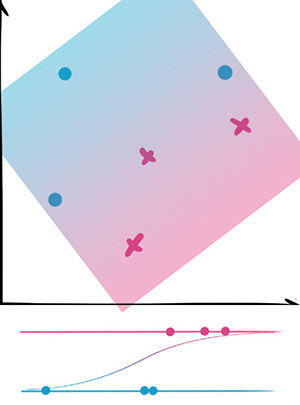
\includegraphics[width=0.5\textwidth]{figure/lr-model.jpg}
    \caption{Ligistic Regression Classification}
\end{figure}

\subsubsection{Train}
set fold of cross validataion to 10

Average Accuracies:  0.7616352201257862

Standart Deviation Accuracies:  0.048131816098786834

\subsubsection{Test}
Test Accuracy 0.7445887445887446

The confusion matrix:
\begin{figure}[H]
    \centering
    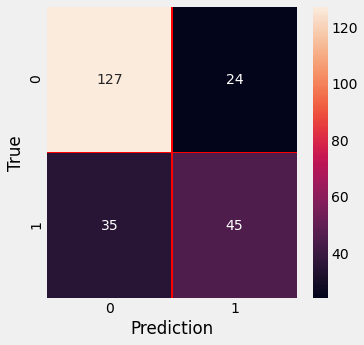
\includegraphics[width=0.4\textwidth]{figure/conmat-lr.png}
    \caption{confusion matrix of logistic regression classification}
\end{figure}

\subsection{K-NN}
\subsubsection{Description}
 KNN is the typical example of Nearest Neighbor Algorithm, and its idea is-for the point to be determined, find the closest data points to it and determine the type of the point to be determined according to their type.

 \begin{figure}[H]
    \centering
    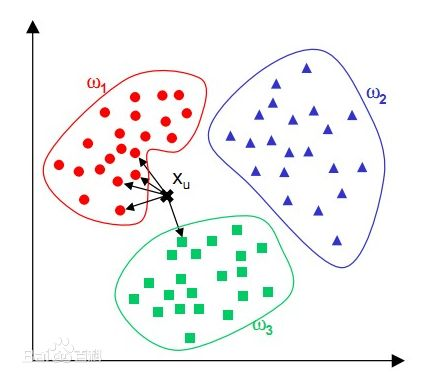
\includegraphics[width=0.4\textwidth]{figure/knn-model.jpg}
    \caption{K-NN model}
\end{figure}
It is characterized by completely following the data, there is no mathematical model at all.

When a particularly easy to explain model is needed, KNN should be used. 

For example, a recommendation algorithm that needs to explain the reason to the user.

\subsubsection{Optimize K}
We iterate the k to get the optimum k:
\begin{figure}[H]
    \centering
    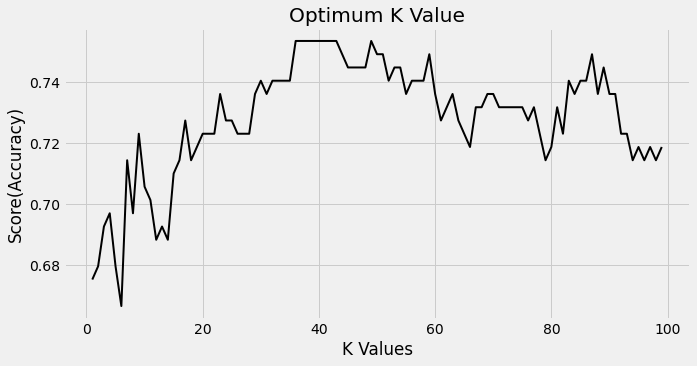
\includegraphics[width=0.8\textwidth]{figure/opti-k.png}
    \caption{optimum K}
\end{figure}
\subsubsection{Train}
set fold of cross validataion to 10 and k = 40

Average Accuracies:  0.7431167016072676

Standart Deviation Accuracies:  0.04692037472446394

\subsubsection{Test}
40-NN Score: 0.7532467532467533

The confusion matrix:
\begin{figure}[H]
    \centering
    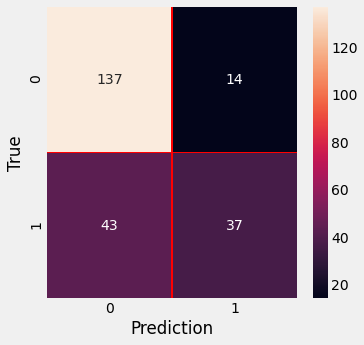
\includegraphics[width=0.4\textwidth]{figure/conmat-knn.png}
    \caption{confusion matrix of knn}
\end{figure}

\subsection{SVM}
\subsubsection{Decription}
A support vector machine takes these data points and outputs the hyperplane (which in two dimensions it’s simply a line) that best separates the tags. This line is the decision boundary: anything that falls to one side of it we will classify as blue, and anything that falls to the other as red.

The core idea of ​​SVM is to find the interface between different categories, so that the two types of samples fall on both sides of the surface as far as possible, and as far as possible from the interface.
\begin{figure}[H]
    \centering
    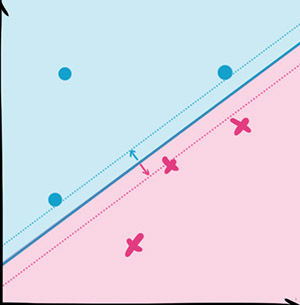
\includegraphics[width=0.35\textwidth]{figure/svm-model.jpg}
    \caption{svm model}
\end{figure}
The earliest SVMs were flat and very limited. But using the kernel function, we can map the plane into a curved surface, which greatly improves the scope of SVM.
\begin{figure}[H]
    \centering
    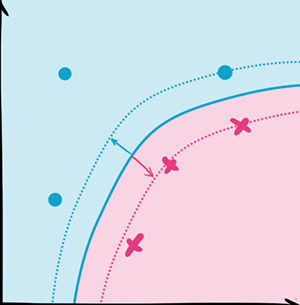
\includegraphics[width=0.35\textwidth]{figure/svm-model2.jpg}
    \caption{svm model with kernel function}
\end{figure}

SVM has excellent performance on many data sets. Relatively speaking, the nature of SVM to keep the distance to the sample as much as possible makes it more resistant to attack.

Like Random Forest, this is an algorithm that you can try before you get the data.

\subsubsection{Train}
set fold of cross validataion to 10, we get

Average Accuracies:  0.76722571628232

Standart Deviation Accuracies:  0.055156325649035956

\subsubsection{Test}
SVM Accuracy: 0.7532467532467533

The confusion matrix:
\begin{figure}[H]
    \centering
    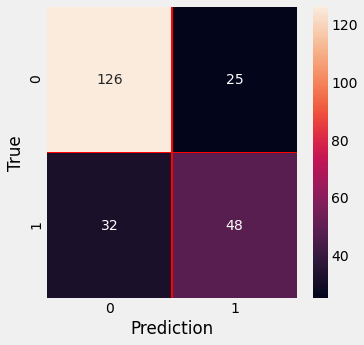
\includegraphics[width=0.35\textwidth]{figure/conmat-svm.png}
    \caption{confusion matrix of svm}
\end{figure}

\subsection{Naive Bayes Classification}
\subsubsection{Description}
Abstractly, naive Bayes is a conditional probability model: given a problem instance to be classified.

The core idea is to calculate the type of point to be judged based on conditional probability.
It is a relatively easy-to-understand model that is still used by spam filters.

When you need a model that is easier to explain and has less correlation between different dimensions. High-dimensional data can be processed efficiently, although the results may not be satisfactory.

\begin{figure}[H]
    \centering
    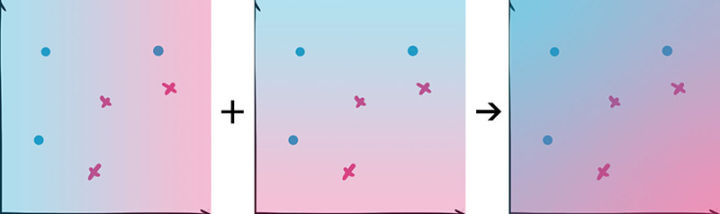
\includegraphics[width=0.4\textwidth]{figure/nby-model}
    \caption{naive bayes model}
\end{figure}

\subsubsection{Train}
set fold of cross validataion to 10, we get

Average Accuracies:  0.7577218728162125

Standart Deviation Accuracies:  0.056690670157824676

\subsubsection{Test}
Accuracy of Naive Bayes Score:  0.7445887445887446
The confusion matrix:
\begin{figure}[H]
    \centering
    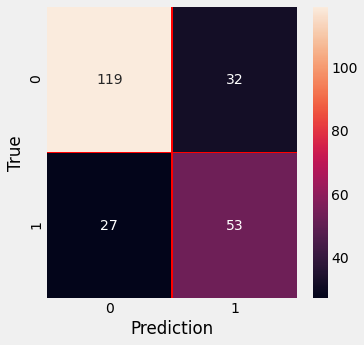
\includegraphics[width=0.4\textwidth]{figure/conmat-nb.png}
    \caption{confusion matrix of naive bayes}
\end{figure}

\subsection{Decision Tree}
\subsubsection{Description}
A decision tree is drawn upside down with its root at the top. In the image on the left, the bold text in black represents a condition/internal node, based on which the tree splits into branches/ edges. The end of the branch that doesn’t split anymore is the decision/leaf, in this case, whether the passenger died or survived, represented as red and green text respectively.

A real dataset will have a lot more features and this will just be a branch in a much bigger tree, but you can’t ignore the simplicity of this algorithm. The feature importance is clear and relations can be viewed easily. This methodology is more commonly known as learning decision tree from data and above tree is called Classification tree as the target is to classify passenger as survived or died. Regression trees are represented in the same manner, just they predict continuous values like price of a house. In general, Decision Tree algorithms are referred to as CART or Classification and Regression Trees.

\begin{figure}[H]
    \centering
    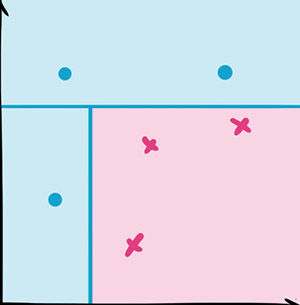
\includegraphics[width=0.4\textwidth]{figure/dt-model}
    \caption{decision tree model}
\end{figure}
Because it can generate a clear tree structure that selects different prediction results based on features, data analysts often use decision trees when they want to better understand the data at hand. It is also a classifier that is relatively easy to be attacked [3]. The attack here refers to artificially changing some characteristics, making the classifier judge wrong. Commonly seen in spam avoidance detection. Because the final decision of the decision tree at the bottom is based on a single condition, the attacker often only needs to change very few features to escape the monitoring. Limited by its simplicity, the greater use of decision trees is the cornerstone of some more useful algorithms.

\subsubsection{Train}
set fold of cross validataion to 10, we get

Average Accuracies:  0.709329140461216

Standart Deviation Accuracies:  0.08114324756907662

\subsubsection{Test}
Decision Tree Score:  0.7012987012987013

The confusion matrix:
\begin{figure}[H]
    \centering
    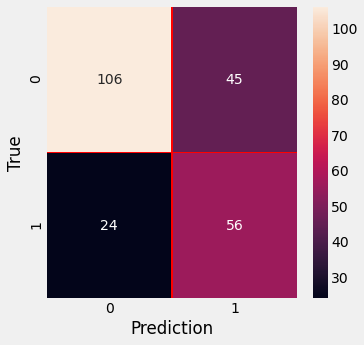
\includegraphics[width=0.4\textwidth]{figure/conmat-dt.png}
    \caption{confusion matrix of decision tree}
\end{figure}



\subsection{Random Forest}
\subsubsection{Description}
Strictly speaking, random forest is actually an integrated algorithm. It first randomly selects different features and training samples to generate a large number of decision trees, and then synthesizes the results of these decision trees to make the final classification. Random forests are widely used in reality analysis. Compared with decision trees, they have greatly improved the accuracy, and at the same time improved the characteristics of decision trees that are easily attacked.
\begin{figure}[H]
    \centering
    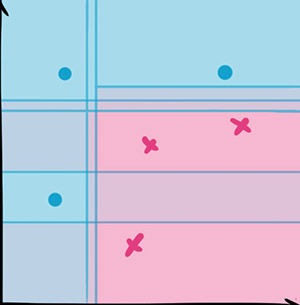
\includegraphics[width=0.4\textwidth]{figure/rf-model.jpg}
    \caption{random forest model}
\end{figure}

When the data dimension is relatively low (several tens of dimensions), and at the same time has high requirements for accuracy.

Because it don't need a lot of parameter adjustments to achieve good results, researcher can try random forest first if you don't know what method to use.


\subsubsection{Optimize N}
iterate N to get optimum N-Estimator

\begin{figure}[H]
    \centering
    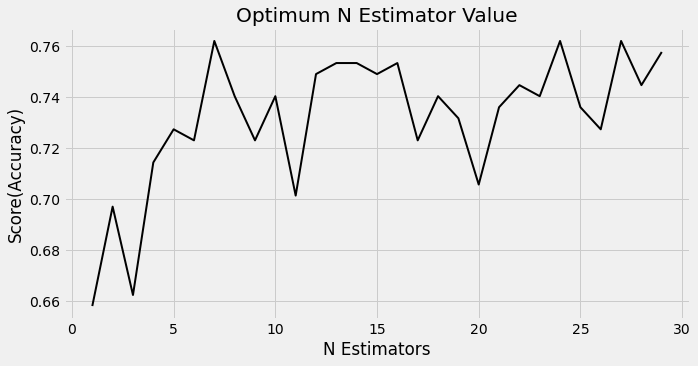
\includegraphics[width=0.4\textwidth]{figure/rf-opti-n.png}
    \caption{optimum N-Estimator}
\end{figure}
\subsubsection{Train}
set fold of cross validataion to 10, estimators-n to 24, we get

Average Accuracies:  0.763487071977638

Standart Deviation Accuracies:  0.04646612575128928

\subsubsection{Test}
Random Forest Score:  0.7705627705627706

The confusion matrix:
\begin{figure}[H]
    \centering
    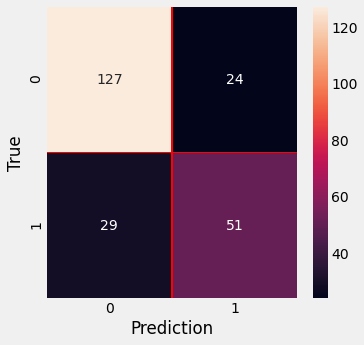
\includegraphics[width=0.4\textwidth]{figure/conmat-rf.png}
    \caption{confusion matrix of random forest}
\end{figure}



\subsection{Gradient Boosting Decision Tree}
\subsubsection{Description}
Boosting method (boosting) In the classification problem, it learns multiple classifiers by changing the weight of training samples (increasing the weight of error-sampling samples and changing the weight of team samples), so that these classifiers are linearly combined to improve classification Performance. 

Gradient Boosting is a Boosting method. Its main idea is that each time the model is established, the gradient descent direction of the model loss function is established before. The loss function is to evaluate the performance of the model (generally the degree of fit + regular term), and the smaller the loss function, the better the performance. And let the loss function continue to decline, so that the model can be continuously modified to improve performance. The best way is to make the loss function fall along the gradient direction (reasonably the fastest decline in the gradient direction). Gradient Boost is a framework in which many different algorithms can be nested.

The lifting method based on the decision tree as the basis function is called lifting tree, and the decision tree can be a classification tree OR regression tree. The lifting tree model can be expressed as an additive model of the decision tree.


\subsubsection{Train}
set fold of cross validataion to 10, we get

Average Accuracies:  0.7504542278127183

Standart Deviation Accuracies:  0.0575141396610466


\subsubsection{Test}
Gradient Boosting Classifier Score 0.7272727272727273

The confusion matrix:
\begin{figure}[H]
    \centering
    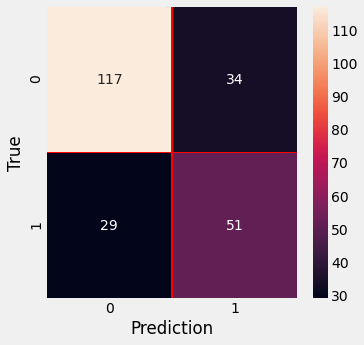
\includegraphics[width=0.4\textwidth]{figure/conmat-gbdt.png}
    \caption{confusion matrix of random forest}
\end{figure}




\subsection{Artificial Neural Network}
\subsubsection{Description}
Its core idea is to use training samples to gradually improve the parameters. As an example of height prediction, if one of the input features is gender (1: male; 0: female), and the output feature is height (1: high; 0: short). Then, when the training sample is a tall boy, in the neural network, the route from "male" to "high" will be strengthened. Similarly, if a tall girl comes, the route from "female" to "high" will be strengthened. 

In the end, which route of the neural network is stronger is determined by our sample. 

The advantage of a neural network is that it can have many, many layers. If the input and output are directly connected, it is no different from LR. But through the introduction of a large number of intermediate layers, it can capture the relationship between many input features. Convolutional neural networks have a classic visualization of different layers (visulization), I will not repeat them here. The neural network is actually proposed very early, but its accuracy depends on the huge training set, which was originally limited by the speed of the computer, and the classification effect has not been as good as the classic algorithms of random forest and SVM.

When the amount of data is huge and there is an internal relationship between the parameters. Of course, now that the neural network is not just a classifier, it can also be used to generate data for dimensionality reduction, which is not discussed here.

\subsubsection{Train}
We use a 5-layer ANN, which take adam as optimizer and binary cross entropy as loss function, to train the data:

\begin{figure}[H]
    \centering
    \begin{neuralnetwork}[height=4]
        \newcommand{\nodetextclear}[2]{}
        \newcommand{\nodetextx}[2]{$x_#2$}
        \newcommand{\nodetexty}[2]{$y_#2$}
        \inputlayer[count=8, bias=false, title=Input\\layer, text=\nodetextx]
        \hiddenlayer[count=8, bias=false, title=Hidden\\layer 1, text=\nodetextclear] \linklayers
        \hiddenlayer[count=8, bias=false, title=Hidden\\layer 2, text=\nodetextclear] \linklayers
        \hiddenlayer[count=8, bias=false, title=Hidden\\layer 2, text=\nodetextclear] \linklayers
        \outputlayer[count=1, title=Output\\layer (Hidden), text=\nodetexty] \linklayers
    \end{neuralnetwork}
    \caption{ANN}
\end{figure}

\begin{figure}[H]
    \centering
    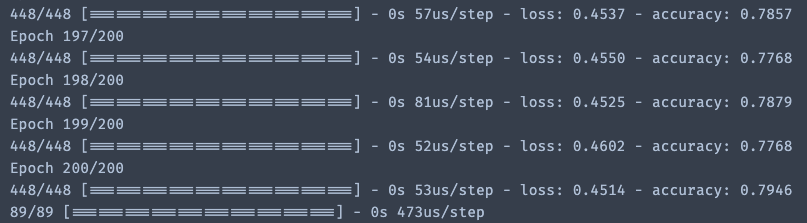
\includegraphics[width=1.0\textwidth]{figure/ann.png}
    \caption{Epoch = 200}
\end{figure}

Accuracy mean: 0.722659170627594

Accuracy variance: 0.07086206094228635
\subsubsection{Test}


ANN Score: 0.7056276798248291

The confusion matrix:
\begin{figure}[H]
    \centering
    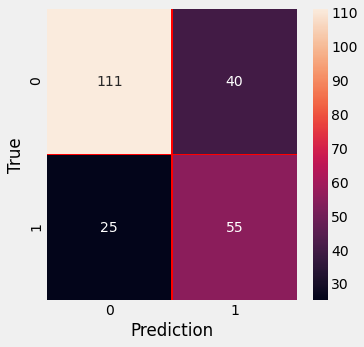
\includegraphics[width=0.4\textwidth]{figure/conmat-ann.png}
    \caption{confusion matrix of artificial neural network}
\end{figure}


\section{Evaluation}
The traditional F-measure or balanced F-score (F1 score) is the harmonic mean of precision and recall.
The number of positive sample is $P$, The number of negative sample is $N$

The recognition rate $Acc=\frac{TP+TN}{TP+TN+FP+FN}=\frac{TP+TN}{P+N}$

$\text{Recall}=\frac{TP}{TP+FN}=\frac{TP}{P}$

$\text{Precision}=\frac{TP}{TP+FP}$

$F_1=\frac{2 T P}{2 T P+F N+F P}=\frac{2 \cdot \text { Precision } \cdot \text { Recall}}{\text {Precision }+\text { Recall}}$

Recall reflects the classification model H's ability to identify positive samples. The higher the recall, the stronger the model's ability to identify positive samples. Precision reflects the model's ability to distinguish negative samples. The higher the precision, the better the model's discrimination of negative samples. The stronger the ability. F1-score is a combination of the two. The higher the F1-score, the more robust the classification model. Therefore, We take F1-Score as the pivot factor:

We get the f1-score table:


\begin{table}[H]
    \centering
    \begin{tabular}{|l|l|}
    \hline
    Algorithm           & f1-score           \\ \hline
    Logistic Regression & 0.7396488695457325 \\ \hline
    K-NN                & 0.7367438032321222 \\ \hline
    SVM                 & 0.7503970108196265 \\ \hline
    Naive Bayes         & 0.7463086857026251 \\ \hline
    Decision Tree       & 0.7074652407618727 \\ \hline
    Random Forest       & 0.7687305514351853 \\ \hline
    Gradient Boosting Decision Tree      & 0.72910927456382 \\ \hline
    Artificial Neural Network     & 0.7233208139131484 \\ \hline
    \end{tabular}
    \caption{F1-score of algorithms}
\end{table}

\section{Conclusion}
Generally speaking, the Logistic Regression, K-NN, SVM, Naive Bayes and Decision Tree need less computation, with time consuming less than 1s. While Gradient Boosting Decision Tree and ANN need more computation with more time. The Random Forest has the best f1-score.

In this dataset, we find some high correlation within some input features, so we can choose the ANN and Gradient Boosting Decision Tree to resist this property.

From the perspective of the accuracy and robustness, the SVM and Random Forest are the best choices.
%\bibliography{wpref}

\end{document}
